\documentclass{standalone}
\usepackage{pgf}
\usepackage[english]{babel}
\usepackage[utf8]{inputenc}
%\usepackage{beamerthemesplit}
\usepackage{graphics,epsfig, subfigure}
\usepackage{url}
\usepackage{srcltx}
\usepackage{hyperref}
\usepackage{mathtools}
\usepackage{amsfonts}
\usepackage{amsmath}
\usepackage{physics}
\begin{document}
$
\begin{aligned}
	A_6^{\text{BCJ},1}&=\raisebox{-5.4mm}{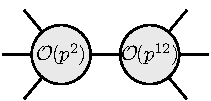
\includegraphics[trim={0cm 0cm 0cm 0cm},clip,scale=0.8]{bcj1-fac}}+\raisebox{-6.5mm}{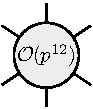
\includegraphics[trim={0cm 0cm 0cm 0cm},clip,scale=0.8]{bcj1-contact}},\\
	A_6^{\text{BCJ},2}&=\raisebox{-5.4mm}{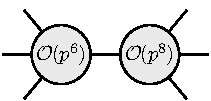
\includegraphics[trim={0cm 0cm 0cm 0cm},clip,scale=0.8]{bcj2-fac}}+\raisebox{-6.5mm}{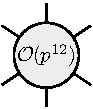
\includegraphics[trim={0cm 0cm 0cm 0cm},clip,scale=0.8]{bcj1-contact}},\\
	A_6^{\text{BCJ},3}&=\raisebox{-6.5mm}{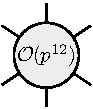
\includegraphics[trim={0cm 0cm 0cm 0cm},clip,scale=0.8]{bcj1-contact}},~~~A_6^{\text{BCJ},4}=\raisebox{-6.5mm}{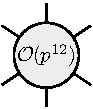
\includegraphics[trim={0cm 0cm 0cm 0cm},clip,scale=0.8]{bcj1-contact}}.
\end{aligned}
$
\end{document}